\documentclass[12pt]{article}

\usepackage{graphicx}
\usepackage{fullpage}
\usepackage[hidelinks]{hyperref}

\begin{document}



\title{US ACARS 3.0 Operating Manual}
\author{Michael Levin}


\includegraphics[scale=1]{Figure1.pdf}
\vspace*{\fill} 


\begin{center}
{\LARGE US ACARS 3 Operating Manual}\\
{\large Version 3.0}\\
\hfill \\ \hfill \\ \hfill \\ \hfill \\ \hfill \\ \hfill \\ 
{\Large Michael Levin}\\
Senior Vice President of Operations\\

\hfill \\ \hfill \\ \hfill \\ \hfill \\
\today
\end{center}

\vspace*{\fill} \newpage

\tableofcontents

\newpage

\section{Legal information and disclosure}
The US Airways logos and trademarks on this site remain the property of US Airways. USAVA is in no way affiliated with the real world US Airways. There is no trade channel for USAVA. The web-site is for entertainment and education and not for a commercial purpose. 
No part of the USAVA website design or layout, documents, or software may be reproduced or transmitted in any form or by any other means electronic or mechanical to include photocopying, recording, reproducing, or electronic storage. Any such act represents a copyright violation and theft of intellectual property solely owned by US Airways Virtual Airways.

\section{Introduction}
Welcome to US Airways Virtual Airlines. The purpose of this guide is to familiarize you with our custom pilot reporting software, US ACARS. This program is offered for free to all registered USAVA pilots, and is the preferred option for filing pilot reports (PIREPs). Additionally, US ACARS provides real-time messaging with other online USAVA pilots.

ACARS is the Aircraft Communications Addressing and Reporting System. US ACARS has two components fulfilling this system. First, ACARS records data from your aircraft every 15 seconds, including fuel, airspeed, position, landing rates, and more. This data is used by PIREP reviewers to determine the approval / rejection decisions and provide feedback on your airmanship. Second, ACARS provides a chat service as well as status of other company flights.

\subsection{Systems requirements}
The following software is required for use of US ACARS 3.0.

\begin{itemize}
\item{Microsoft Windows XP / VISTA / 7 / 8}
\item{Microsoft Flight Simulator 2002 / 2004 / 9 / X \textbf{or} XPlane 9 / 10 \textbf{or} Prepar3d}
\item{FSUIPC \textbf{or} XPUIPC}
\end{itemize}

US ACARS 3.0 has not been tested on Mac or Unix systems, but as it the program is platform-independent it may be able to run successfully.

\subsection{Changes from US ACARS 2.2}
This section lists additional features included in US ACARS 3.0 beyond those in US ACARS 2.2.

\subsubsection*{User interface changes}
\begin{itemize}
\item{Color-coded messages – chat messages are color-coded depending on type.}
\item{Prompt on exit – when in flight, ACARS will provide a dialogue box to confirm exiting to avoid loss of flight recording.}
\item{The online members list updates instantly when pilots connect or disconnect, or their flight status changes.}
\item{Complete itinerary – any flights on your itinerary can be loaded into the dispatch panel.}
\item{Weather reports – the “weather” tab provides METARs and TAFs for any airport.}
\end{itemize}

\subsubsection*{Flight recording modifications}
\begin{itemize}
\item{Bounce protection – ACARS will ignore bounces. Aircraft must stay in the air 5 seconds after takeoff, and remain on the ground 5 seconds after landing, to register a takeoff or landing event.}
\item{Pause detection – ACARS does not add flight time when the simulator is paused. Additionally, exceeding the limit on breaks will result in a comment being added to notify PIREP reviewers.}
\item{Offline flight recording – ACARS can be started offline and used to record PIREPs. PIREPs are automatically submitted when a connection is made.}
\item{Elimination of ACARS manual PIREPs – if PIREP submission fails, ACARS will re-send the PIREP when the server is available.} 
\end{itemize}

\subsubsection*{Other features}
\begin{itemize}
\item{Private messaging. Members can send messages to specific pilots or to all staff.}
\item{Muting: staff members can mute pilots to prevent them from sending messages to other pilots.}
\item{PIREPs are encrypted, so XML files cannot be sent independently to USAVA staff. XML files cannot be read or modified intelligently without the decryption key.}
\item{Security of network communications has been improved.}
\end{itemize}

\section{Installation}

\subsection{US ACARS 3}
US ACARS 3 is distributed as a packaged installer. Simply follow the instructions in the installation wizard to install US ACARS.

\begin{center}
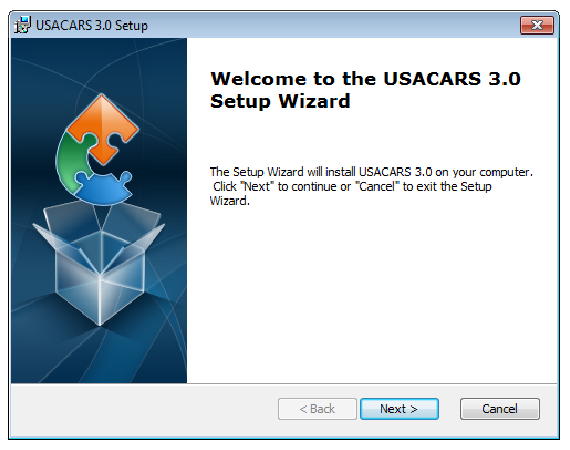
\includegraphics[scale=1]{Image1.pdf}
\end{center}

US ACARS 3 also requires the latest version of FSUIPC or XPUIPC. See sections 3.2 and 3.3, respectively.

\subsection{FSUIPC}
Download the latest version of FSUIPC from \url{http://www.schiratti.com/dowson.html}.

\subsection{XPUIPC}
Download the latest version of XPUIPC from \url{http://www.tosi-online.de/XPUIPC/XPUIPC.html}.

\section{Connecting to ACARS}
When you open US ACARS 3, you will be taken to the login screen:


\begin{center}
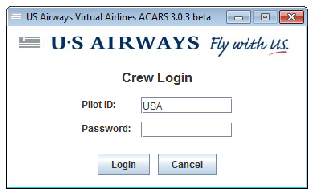
\includegraphics[scale=1]{Image2b.pdf} \hfill 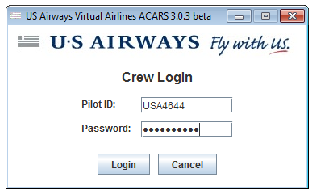
\includegraphics[scale=1]{Image2c.pdf}
\end{center}

Enter your pilot ID and password to continue.
If the server is unavailable, you will see a connecting to server message while the client attempts to connect, followed by a notification that offline mode has been activated.

\begin{center}
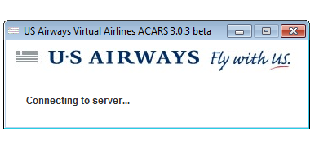
\includegraphics[scale=1]{Image3.pdf}
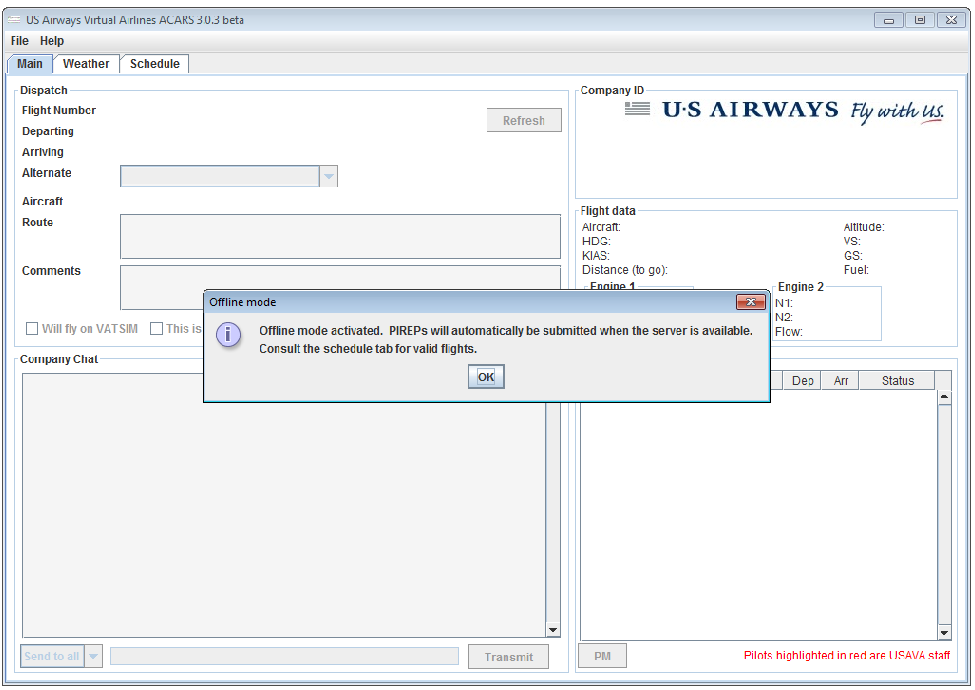
\includegraphics[scale=1]{Image4.pdf}
\end{center}

In offline mode, chat messages and online status are disabled, and the schedule tab appears, instead of the itinerary tab. The itinerary and schedule panels are described in more detail in Sections 5.7 and 5.8, respectively.

\section{US ACARS 3 interface}

\begin{center}
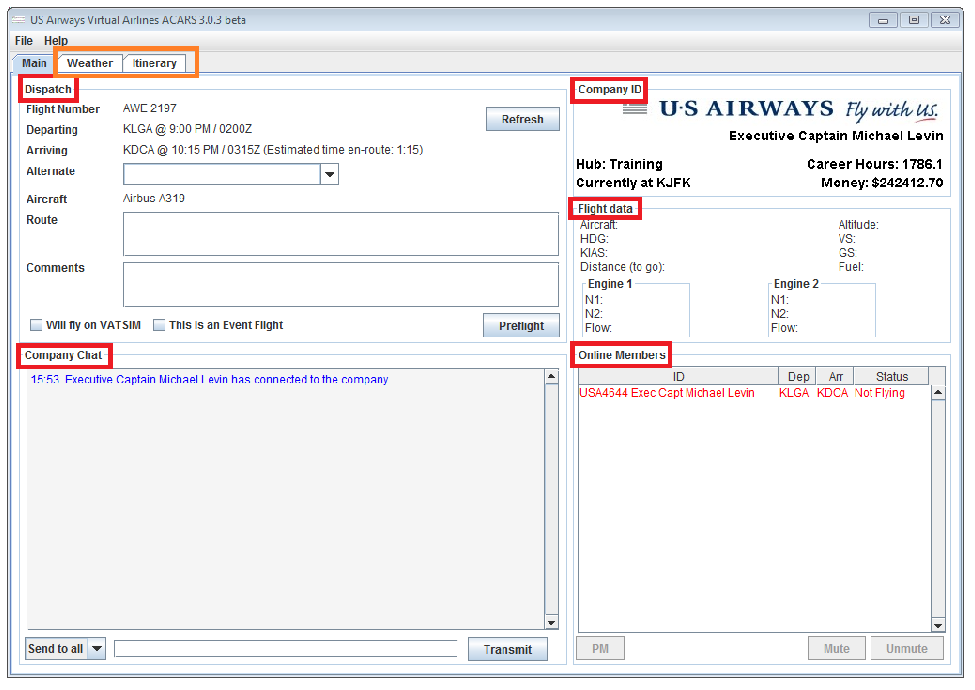
\includegraphics[scale=1]{Image5.pdf}
\end{center}

\subsection{Dispatch panel}
The dispatch panel shows the current flight you have loaded.

\begin{center}
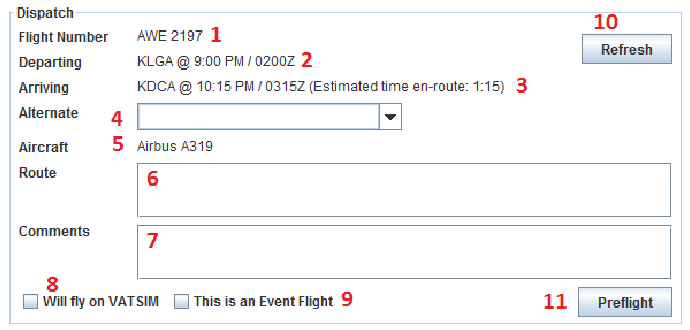
\includegraphics[scale=1]{Image6.pdf}
\end{center} 

\begin{enumerate}
\item{The flight number shows both the carrier and the US Airways / American Airlines flight number (which may be a codeshare number). }
\item{The departing field gives the ICAO code of the origin airport, followed by the scheduled departure time in local and GMT. }
\item{Similarly, the arriving field gives the ICAO code of the destination airport, followed by the scheduled arrival time in local and GMT, with the expected gate-to-gate time in parentheses.}
\item{The alternate field allows you to choose an alternate airport from among the list of all airports in the database.}
\item{The aircraft field shows the scheduled equipment of the loaded flight. See the Aircraft Operations Handbook for permitted substitutions.}
\item{The route field is where you enter the planned route for your flight. Note that you can only modify the route before pressing “preflight”.}
\item{Comments can be added at any time during the flight, and are used to make notes about the flight or communicate with PIREP reviewers.}
\item{Check the “Will fly on VATSIM” checkbox if you are flying on VATSIM or IVAO.}
\item{Check the “This is an Event flight” checkbox if the flight is a USAVA or VATSIM event flight.}
\item{If you modify your itinerary through the USAVA website, click the refresh button to update ACARS with the new itinerary.}
\item{This is the action button. Depending on the stage of flight, it displays “preflight”, “begin flight”, or “end flight”. ACARS procedures are discussed in more detail in section 6.}
\end{enumerate}

\subsection{Company information}

\begin{center}
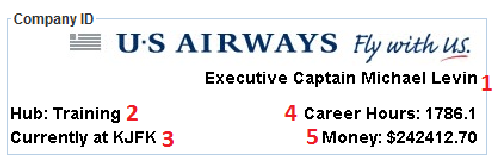
\includegraphics[scale=1]{Image7.pdf}
\end{center} 

\begin{enumerate}
\item{Your rank at USAVA}
\item{Your current hub}
\item{Your last location, based on the last approved PIREP. If your next flight does not depart from your last location, you may be assessed a jumpseat fee.}
\item{Your career hours with USAVA. This is one of the factors affecting promotion.}
\item{Your career money with USAVA. Money is accrued by flying and lost through jumpseating.}
\end{enumerate}

\subsection{Flight data recorder}

Most of the flight data is fairly self-explanatory, but two items are noteworthy:

\begin{center}
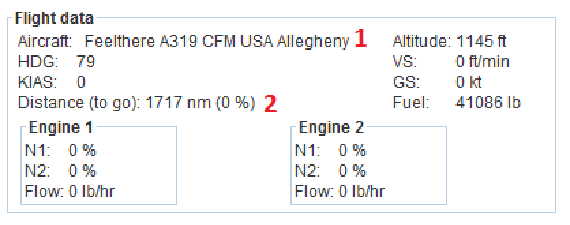
\includegraphics[scale=1]{Image8.pdf}
\end{center} 

\begin{enumerate}
\item{The title of your aircraft. Check this to ensure that you are flying the correct equipment type as scheduled.}
\item{Distance to go is measured from your aircraft’s current position to the location of the destination.}
\end{enumerate}

\subsection{Company chat}

\begin{center}
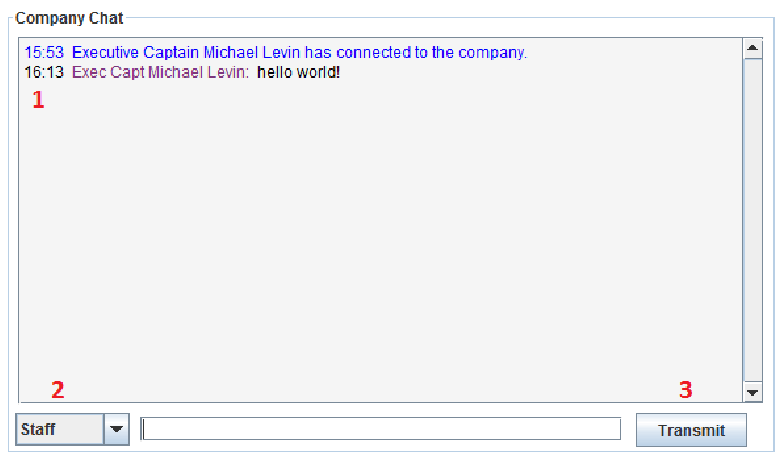
\includegraphics[scale=1]{Image9.pdf}
\end{center} 

\begin{enumerate}
\item{This is the chat log. Messages are color-coded depending on type. 
\begin{enumerate}
\item{Blue - pilot connect/disconnect}
\item{Green - takeoff / landing event }
\item{Black - chat }
\item{Orange - private message}
\item{Red - staff message or announcement}
\end{enumerate}
}
\item{This drop-down box selects the recipient of your message. Send to all is the default, although you can also choose to message staff or private message another pilot (see section 5.5). Staff members may send announcements, which appear in red.}
\end{enumerate}

\subsection{Online status}
\begin{center}
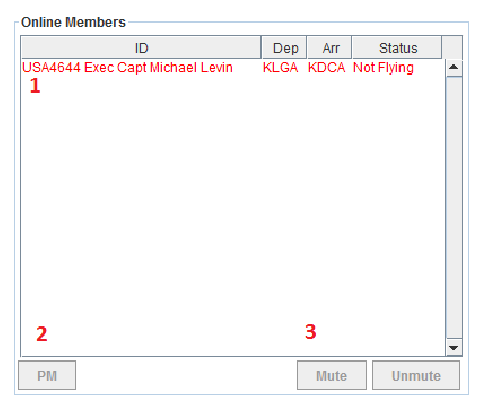
\includegraphics[scale=1]{Image10.pdf}
\end{center} 

\begin{enumerate}
\item{This is a list of online members. Staff members’ names appear in red.}

\item{The PM button allows you to PM other members. If you select a member other than yourself, the PM button will be enabled, and clicking it will add the member to the recipient selection in the chat panel.}

\item{Staff members can mute or unmute other pilots. These two buttons only appear for staff members.}
\end{enumerate}

\subsection{Weather}
The weather tab retrieves the latest METAR and TAF from Aviation Digital Data Services.

\begin{center}
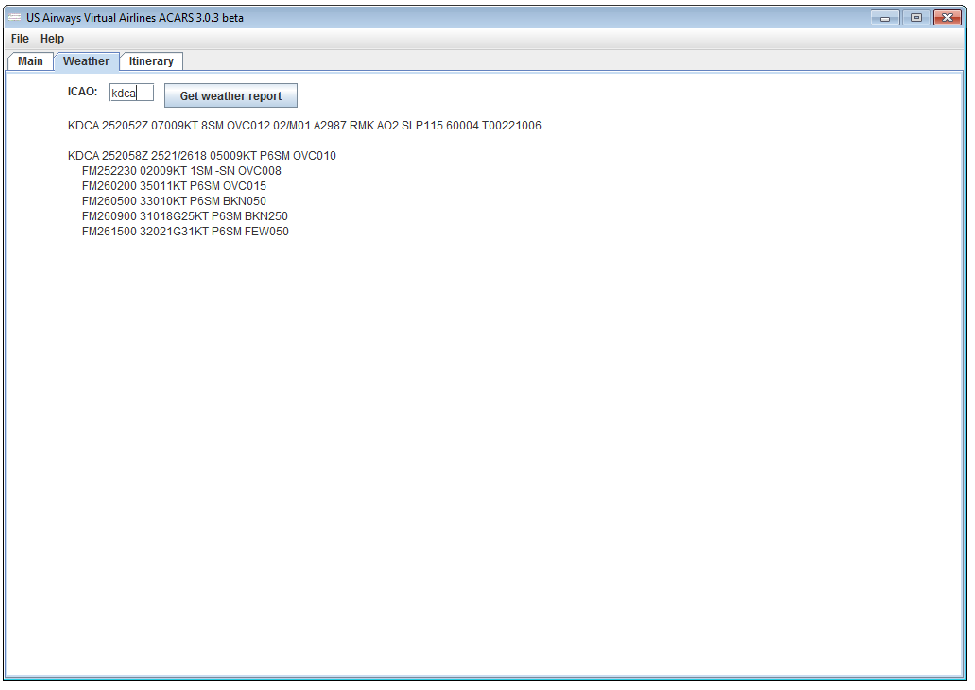
\includegraphics[scale=1]{Image11.pdf}
\end{center} 

\subsection{Current itinerary}
The itinerary tab shows you all flights you have booked from the website. You can load any of these into the dispatch panel by pressing “select flight”. Pressing the refresh button on the dispatch panel will reload your itinerary. You also have the option of searching for flights; the options are the same as on the website.

\begin{center}
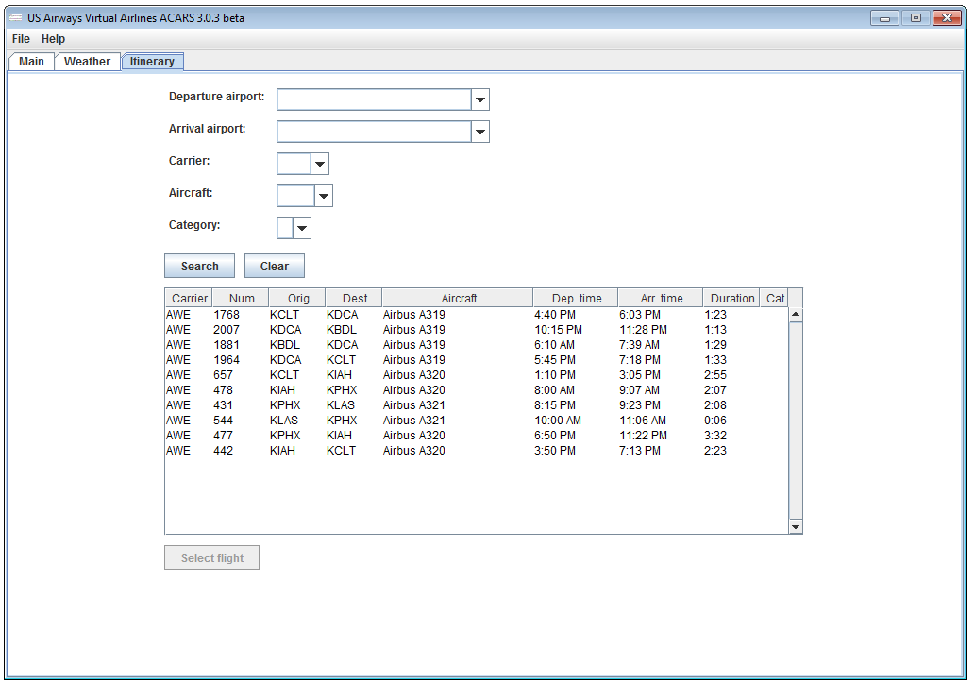
\includegraphics[scale=1]{Image12.pdf}
\end{center} 

The schedule tab may not be able to check your rank against the required rank to fly a flight. If not, it will display a warning. Even if you can select the flight, it is your responsibility to ensure that you have sufficient rank to fly it.


\section{Flight procedures}
This section describes the procedures for recording a flight through ACARS. Section 6.4 has checklists for use with flight.

\subsection{Preflight}
Before starting a flight, select the alternate airport, enter in the planned route, and check the VATSIM and event checkboxes if appropriate.

\begin{center}
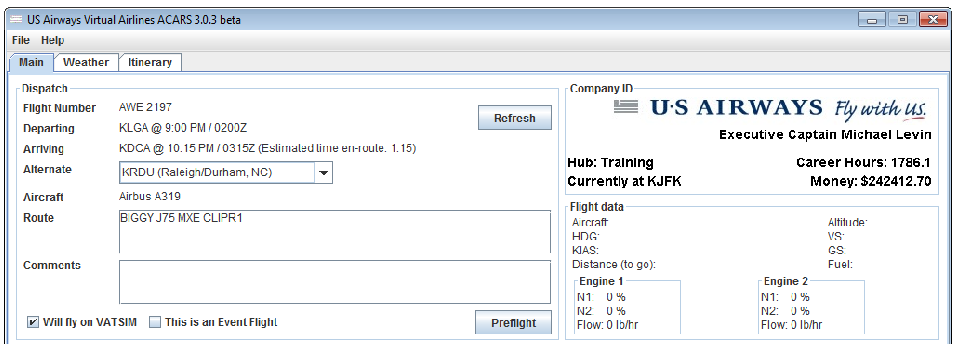
\includegraphics[scale=1]{Image13.pdf}
\end{center} 

Load flight simulator with your aircraft parked at the gate, with parking brakes on. Press “preflight” to connect US ACARS to your aircraft.

\begin{center}
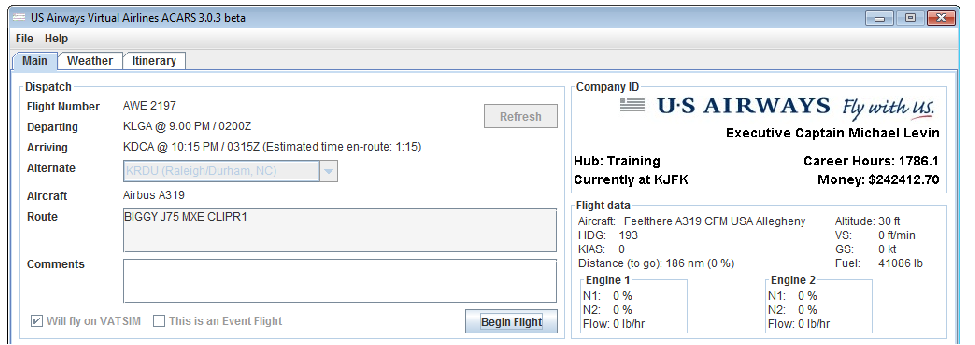
\includegraphics[scale=1]{Image14.pdf}
\end{center} 

Notice that you can no longer modify the alternate airport, route, and VATSIM and event checkboxes. You should also see flight data. Check that the aircraft you’re flying is the correct type.

\subsection{Begin flight}
After loading your aircraft with fuel, when you are ready to pushback from the gate, select “begin flight”. The action button will now display “end flight”.

\begin{center}
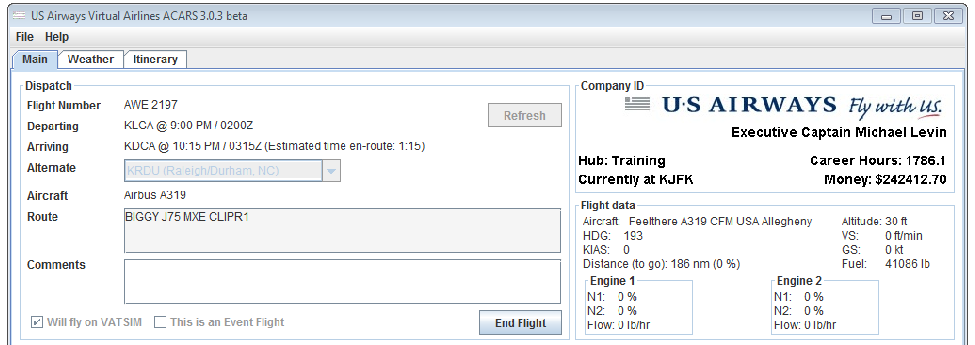
\includegraphics[scale=1]{Image15.pdf}
\end{center} 

\subsection{End flight}
After you land, park at the gate, shut down engines, and open the doors to allow passengers to exit, press “end flight”. You will be shown a summary of the flight, and asked whether you want to file a PIREP.

\begin{center}
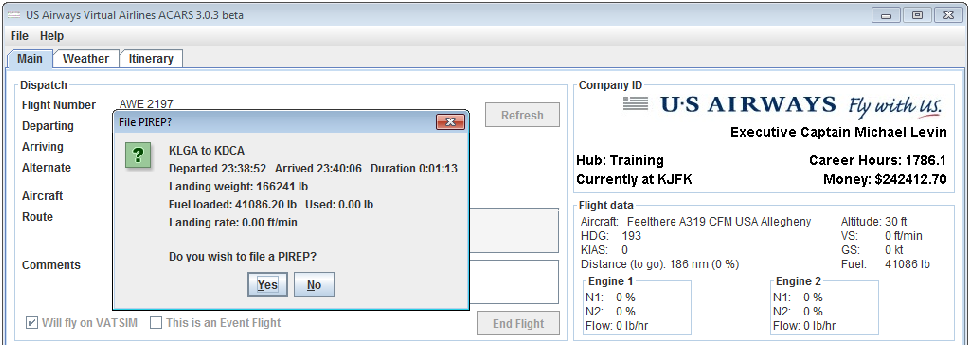
\includegraphics[scale=1]{Image16.pdf}
\end{center} 

\subsection{US ACARS 3 checklists}

\subsubsection*{Preflight}
\begin{tabular}{ll}
Departure airport & CHECK\\
Arrival airport & CHECK\\
Equipment & CHECK\\
Alternate airport & ENTERED\\
Route & ENTERED\\
VATSIM flight & as needed\\
Event flight & as needed\\
Comments & as needed\\
ACARS preflight & SELECT\\
Flight data recorder & CHECK\\
\end{tabular}

\subsubsection*{Before pushback}
\begin{tabular}{ll}
Fuel loaded & CHECK\\
ACARS begin flight & SELECT\\
Pushback & request\\
\end{tabular}

\subsubsection*{After landing and parking at the gate}
\begin{tabular}{ll}
Engines shutdown & CHECK\\
Jetway & as needed\\
Exit open & CHECK\\
ACARS end flight & SELECT\\
ACARS file PIREP & SELECT\\
\end{tabular}

\section{Frequently asked questions}
\begin{enumerate}
\item{\textbf{There’s no one online / I see pilots on US ACARS 2.2 who aren’t on US ACARS 3.}\\
US ACARS 3 uses a completely new server engine that is incompatible with US ACARS 2.2. As a result, chat and members online from US ACARS 2.2 are not shown. }
\item{\textbf{I found a glitch / error. What do I do?}\\
Email the developer at \url{michael.levin@usairwaysva.org}:
\begin{enumerate}
\item{Attach a screenshot of US ACARS 3 at the time of the error}
\item{Describe the conditions / what you were doing leading up to the error}
\item{Look in the "Documents/USACARS/" folder, and attach the "log\_out.txt" and "log\_error.txt" files.}
\end{enumerate}
}
\item{\textbf{I have an old version. How do I update?}\\
Download USACARS3 from \url{http://www.usairwaysva.org/uploads/acars3/usacars.msi}}
\item{\textbf{ACARS 3 cannot connect to flight simulator.}\\
Check that you have the latest version of FSUIPC and XPUIPC installed.}
\item{\textbf{The website is up, but ACARS 3 cannot connect.}\\
Make sure your firewall is not blocking ACARS 3, and is allowing connections through ports 1613 and 1614. You may need to enable port forwarding on those ports in your router.}
\item{\textbf{How do I submit a manual PIREP?}\\
You cannot submit manual PIREPs with US ACARS 3. PIREPs filed offline will be automatically submitted when the server is back online.}
\item{\textbf{ACARS 3 has been downloading the schedule for a few minutes.}\\
Every month, when the schedule is updated, ACARS 3 must download the latest version of the schedule to allow flying offline. The schedule is large, so it may require a few minutes. Do not interrupt this process by exiting US ACARS 3. If a connection problem occurs, US ACARS 3 will terminate by itself. }
\item{\textbf{Could you add a feature?} \\
Email the developer at \url{michael.levin@usairwaysva.org}. However, we reserve the right not to add the feature.}
\item{\textbf{Can I assist with development?}\\
US ACARS 3 is written in Java. If you would like to help, email the developer at \url{michael.levin@usairwaysva.org}.}
\end{enumerate}

















\end{document}